\documentclass{amsart}
\usepackage{amsfonts} % For math fonts
\usepackage{amsmath, amssymb, amsthm}
\usepackage{float}
\usepackage{enumitem}
\usepackage{graphicx}
\setlist[enumerate,1]{label=\arabic*.}
\setlist[enumerate,2]{label=\alph*.,itemindent=2em}
\setlist{topsep=0pt, leftmargin=*, labelsep=1em}


\usepackage{listings}
\usepackage{xcolor}

\lstset{
    language=Python,
    backgroundcolor=\color{black}, % Light gray background
    basicstyle=\ttfamily\small\color{white}, % Code style
    keywordstyle=\color{cyan}\bfseries, % Keywords style
    stringstyle=\color{yellow}, % Strings style
    commentstyle=\color{gray}, % Comments style
    frame=single, % Box around code
    rulecolor=\color{white}, % Frame color
    numbers=left, % Line numbers
    numberstyle=\tiny\color{white}, % Line number style
    breaklines=true, % Automatic line breaking
    showstringspaces=false
}


\title{HW 5 - 151A}
\author{Asher Christian 006-150-286}
\date{ 20.02.25}

\begin{document}
    \maketitle
    \section{Exercise 1}
    \emph{
        Let $f \in C^{4}([a,b]).$ 
        \begin{enumerate}[label  = (\alph*)]
            \item Write down the third order Taylor expansion for $f(x)$
                about the point $x_0 \in (a,b)$. The remainder term
                should be in Mean-value form (Lagrange form)
            \item Use the result from (a) to evaluate $f(x)$ at the points $x = x_0 + h$ and
                $x = x_0-h$. Add the two results together to derive the centered difference approximation to the second derivative:
                \[
                    \frac{f(x_0+h) - 2f(x_0) + f(x_0-h)}{h^2} = f''(x_0) + \frac{h^2}{4!}(f^{(4)}(\xi_1) + f^{(4)}(\xi_2))
                .\]
        \end{enumerate}
    }
    \[
    f(x) = f(x_0) +  f'(x_0)(x-x_0) + \frac{f''(x_0)}{2}(x-x_0)^2 + \frac{f^{(3)}(x_0)}{6}(x-x_0)^{3} + \frac{f^{(4)}(\xi)}{24}(x-x_0)^{4}
    .\] 
    \[
    f(x_0+h) = f(x_0) +  f'(x_0)h + \frac{f''(x_0)}{2}h^2 + \frac{f^{(3)}(x_0)}{6}h^{3} + \frac{f^{(4)}(\xi)}{24}h^{4}
    .\] 
    \[
        \frac{f(x_0+h) - f(x_0)}{h} =  f'(x_0) + \frac{f''(x_0)}{2}h + \frac{f^{(3)}(x_0)}{6}h^{2} + \frac{f^{(4)}(\xi)}{24}h^{3}
    .\] 
    \[
    f(x_0-h) = f(x_0) +  f'(x_0)(-h) + \frac{f''(x_0)}{2}(-h)^2 + \frac{f^{(3)}(x_0)}{6}(-h)^{3} + \frac{f^{(4)}(\xi)}{24}(-h)^{4}
    .\] 
    \[
        \frac{f(x_0-h)-f(x_0)}{h} = -f'(x_0) + \frac{f''(x_0)}{2}h - \frac{f^{(3)}(x_0)}{6}h^{2} + \frac{f^{(4)}(\xi)}{24}h^{3}
    .\] 
    \[
        \frac{f(x_0+h)-2f(x_0)+f(x_0-h)}{h} = f''(x_0)h + \frac{1}{24}h^{3}(f^{(4)}(\xi_1) + f^{(4)}(\xi_2))
    .\] 
    \[
        \frac{f(x_0+h)-2f(x_0)+f(x_0-h)}{h^2} = f''(x_0) + \frac{1}{24}h^{2}(f^{(4)}(\xi_1) + f^{(4)}(\xi_2))
    .\] 

    \section{Exercise 2}
    \emph{
        Let $f(x) = \sin(x)$. Use the backwards difference formula to approximate $f'(\frac{\pi}{3})$ using $h = 0.1$,
        $h = 0.01$ and $h = 0.001$ and record the absolute error. Present your results with 6 digits after decimal
        How much does the error decrease each time?
    }
    \[
    f'(\frac{\pi}{3})  = 0.5 \approx \frac{f(\frac{\pi}{3}) - f(\frac{\pi}{3}-h)}{h}
    .\] 
    \[
        \frac{\frac{\sqrt{3}}{2} - \sin(\frac{\pi}{3}- 0.1)}{0.1} = 0.542432281058 \; |0.542432281058 - 0.5| = 0.0424322810575
    .\] 
    \[
        \frac{\frac{\sqrt{3}}{2} - \sin(\frac{\pi}{3} - 0.01)}{0.01} = 0.504321757643 \; |0.504321757643 - 0.5| = 0.00432175764299
    .\] 
    \[
     \frac{\frac{\sqrt{3}}{2} - \sin(\frac{\pi}{3}-0.001)}{0.001} = 0.500432929332 \; |0.500432929332 - 0.5| = 0.000432929332439
    .\] 
    Each time the error decreases by a factor of 10 approximately

    \section{Exercise 3}
    \emph{
        Using Taylor's theorem, it can be shown that if $f \in C^{5}([a,b]),$ then the centered 
        difference approximation formula for the first derivative is given by
        \[
        f'(x_0) = \frac{f(x_0+h)-f(x_0-h)}{2h} - (\frac{h^2}{6}f'''(x_0) + \frac{h^{4}}{120}f^{(5)}(\xi))
        .\] 
        \begin{enumerate}[label = (\alph*)]
            \item Re-wriet this formula using step size $\frac{h}{2}$ instead of $h$ 
            \item Multiply your answer from (a) by $4$, subtract (*) from the result, and then divide
                everything by 3. what is the error?
        \end{enumerate}
    }
    \[
    f'(x_0) = \frac{f(x_0+\frac{h}{2}) - f(x_0-\frac{h}{2})}{h} - (\frac{h^2}{24}f'''(x_0) + \frac{h^{4}}{1920}f^{(5)}(\xi))
    .\] 
    \[
    4f'(x_0) = \frac{8f(x_0+\frac{h}{2}) - 8f(x_0-\frac{h}{2})}{2h} - (\frac{h^2}{6}f'''(x_0) + \frac{h^{4}}{480}f^{(5)}(\xi))
    .\] 
    \[
    3f'(x_0) = \frac{8f(x_0+\frac{h}{2}) - 8f(x_0-\frac{h}{2}) - f(x_0+h) + f(x_0-h)}{2h}  + \frac{h^{4}}{120}(f^{(5)}(\xi_1) - \frac{1}{4}(f^{(5)}(\xi_2)))
    .\] 
    \[
    f'(x_0) = \frac{8f(x_0+\frac{h}{2}) - 8f(x_0-\frac{h}{2}) - f(x_0+h) + f(x_0-h)}{6h}  + \frac{h^{4}}{40}(f^{(5)}(\xi_1) - \frac{1}{4}(f^{(5)}(\xi_2)))
    .\] 
    The error is $O(h^{4})$

    \section{Exercise 4}
    \[
    |f'(x_0) - \frac{f(x_0+h)-f(x_0-h)}{2h}| \le \frac{M}{6}h^2
    .\] 
    \[
        M = \max_{x\in[a,b]}|f'''(x)|
    .\] 
    \[
        \tilde{f}(x_0+h) := \text{Fl}(f(x_0+h)), \;\;\;\; \tilde{f}(x_0-h) := \text{Fl}(f(x_0-h))
    .\] 
    \emph{
    and suppose that $\epsilon_1,\epsilon_2$ are the errors
    \[
        f(x_0+h) = \tilde{f}(x_0+h) + \epsilon_1, \;\;\;\; f(x_0-h) = \tilde{f}(x_0-h) + \epsilon_2
    .\] 
    Use the triangle inequality and (1) to show that the error in the centered difference approx in the presence
    of round error satisfies:
    \[
        |f'(x_0) - \frac{\tilde{f}(x_0+h)-\tilde{f}(x_0-h)}{2h}| \le \frac{M}{6}h^2 + \frac{|\epsilon_2-\epsilon_1|}{2h}
    .\] 
    }
    \[
        |f'(x_0) - \frac{\tilde{f}(x_0+h) + \epsilon_1 - \tilde{f}(x_0-h) - \epsilon_2}{2h} | \le \frac{M}{6}h^2
    .\] 
    \[
        |f'(x_0) - \frac{\tilde{f}(x_0+h) - \tilde{f}(x_0-h) }{2h}  + \frac{\epsilon_1-\epsilon_2}{2h}| \le \frac{M}{6}h^2
    .\] 
    since $|a + b| \le |a| + |b|$
    \[
        |f'(x_0) - \frac{\tilde{f}(x_0+h)-\tilde{f}(x_0-h)}{2h}| \le \frac{M}{6}h^2 + \frac{|\epsilon_2-\epsilon_1|}{2h}
    .\] 
    (b).
    $\epsilon = \frac{|\epsilon_2-\epsilon_1|}{2}$
     error on (a,b):
     \[
         |\frac{M}{6}h^2 + \frac{\epsilon}{h}|
     .\] 
     assuming $h > 0$ and since $\epsilon \ge 0$ and $M \ge 0$ the previous is equivalent to
     \[
     \frac{M}{6}h^2 + \frac{\epsilon}{h}
     .\] 
     taking derivative
     \[
     \frac{M}{3}h - \frac{\epsilon}{h^2} = 0
     .\] 
     \[
     \frac{M}{3}h = \frac{\epsilon}{h^2}
     .\] 
     \[
     h^{3} = \frac{3\epsilon}{M}
     .\] 
     \[
         h = \sqrt[3]{\frac{3\epsilon}{M}}
     .\] 
     Quickly testing the derivatives at nearby points shows that this value is indeed a minimum

     \section{Exercise 5}
     \emph{
     Approximate the following integrals using the Trapezoidal rule.
     \begin{enumerate}[label = (\alph*)]
         \item $\int_{0}^{1}x^2e^{-x}dx$ 
         \item $\int_{1}^{1.6}\frac{2x}{x^2-4}dx$
     \end{enumerate}
     }
     \[
     \int_{a}^{b}f(x)dx = \frac{h}{2}f(a) + \frac{h_2}{2}f(b) = E(f)
     .\] 
     \begin{enumerate}[label = (\alph*)]
         \item 
             \[
             \int_{0}^{1}x^2e^{-x}dx \approx \frac{1}{2}0^2e^{0} + \frac{1}{2}1^2e^{-1} = \frac{1}{2e}
             .\] 
         \item 
             \[
             \int_{1}^{1.6}\frac{2x}{x^2-4}dx \approx .3  \frac{2}{-3} + .3 \frac{3.2}{2.56-4} = -0.86666666666
             .\] 
     \end{enumerate}

     \section{Exercise 6}
     \emph{
         Consider the function $f(x) = x^2\ln(x)$ we want to approx the derivative at $x = 2$
         \begin{enumerate}[label = (\alph*)]
             \item Use the first order forward difference scheme
                 \[
                 f'(x) \approx \frac{f(x+h)-f(x)}{h}
                 .\] 
                 to approximate $f'(2)$. The answer should be a function of $h$. In addition
                 compute the true value $f'(2)$
             \item Write a code to find the optimal  $h$ of the form $h = 10^{-n}$ where $n$ is a positive
                 integer. Then find the corresponding error. Here, "optimal" means that the absolute error is minimized.
                 Then plot the error curve w.r.t $h$ in a log-log scale.
             \item From (b), we find an optimal $h = 10^{-n}$. Looking at the graph we plot
                 , we should observe that the optimal $h$ should be between $10^{-n-1}$ and $10^{-n+1}$. Compute
                 and plot the error with $h=10^{-n-1+0.01*m}$ for $m \in \{0,1,2,...,199\}$ in log-log scale and 
                 describe what you observe
         \end{enumerate}
     }
     \begin{enumerate}[label = (\alph*)]
         \item 
             \[
             f'(2) \approx \frac{(2+h)^2\ln(2+h) - 2^2\ln(2)}{h}
             .\] 
             \[
             f'(x) = 2x\ln(x) + x \rightarrow f'(2) = 4\ln(2) + 2 \approx 4.77258872224
             .\] 
         \item 
             \begin{figure}[h]
                 \centering
                 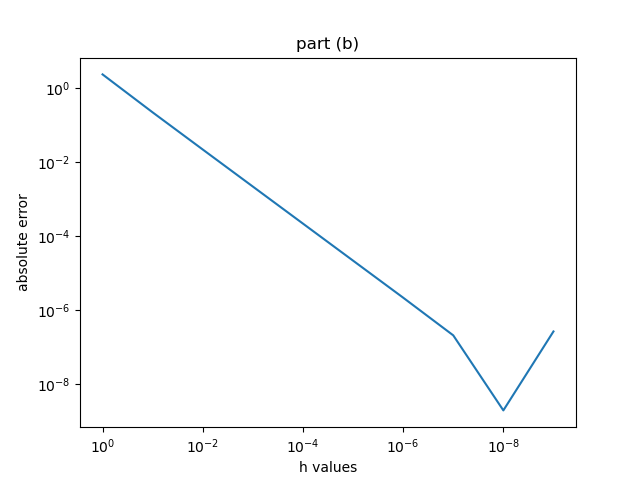
\includegraphics[width=0.8\textwidth]{part_b.png}
             \end{figure}
             \begin{lstlisting}
import matplotlib as plt
import math

import numpy as np
import matplotlib.pyplot as plt

fp = 2*2*np.log(2) + 2
def fp_approx(h):
    return ((((2+h)**2)*(np.log(2+h)))-(4*np.log(2)))/h

error = np.float64('inf')
n = 0
hs = []
errors = []
while True:
    absolute_error = abs(fp-fp_approx(10**(-n)))
    errors.append(absolute_error)
    hs.append(10**(-n))
    n += 1
    if absolute_error > error:
        break
    else:
        error = absolute_error

print(hs)
print(errors)


plt.loglog(hs, errors)
plt.gca().invert_xaxis()
plt.xlabel("h values")
plt.ylabel("absolute error")
plt.title("part (b)")
plt.savefig("part_b.png")
         \end{lstlisting}
         From this we see that the optimal $h$ value of the form  $10^{-n}$ is $10^{-8}$ with corresponding absolute
         error of $1.982478181616898 \times 10^{-9}$
     \item 
         \begin{figure}[h]
             \centering
             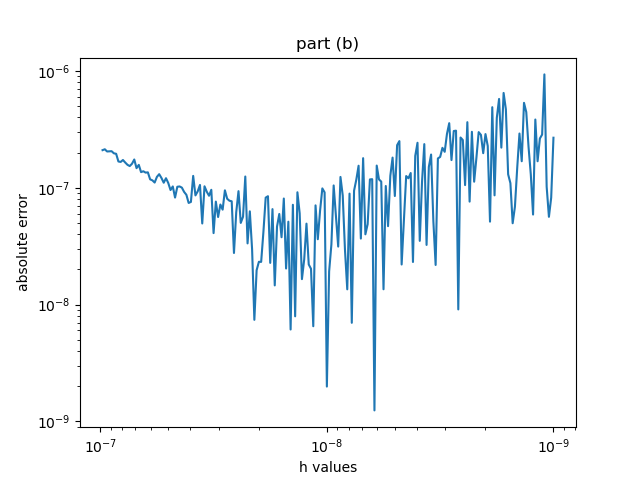
\includegraphics[width=0.8\textwidth]{part_c.png}
         \end{figure}
         \begin{lstlisting}
         \begin{lstlisting}
import matplotlib as plt
import math

import numpy as np
import matplotlib.pyplot as plt

fp = 2*2*np.log(2) + 2
def fp_approx(h):
    return ((((2+h)**2)*(np.log(2+h)))-(4*np.log(2)))/h

n = 8
hs = []
errors = []
for m in range(200):
    h = 10**(-n-1 + 0.01*m )
    absolute_error = abs(fp-fp_approx(h))
    errors.append(absolute_error)
    hs.append(h)

print(hs)
print(errors)


plt.loglog(hs, errors)
plt.gca().invert_xaxis()
plt.xlabel("h values")
plt.ylabel("absolute error")
plt.title("part (b)")
plt.savefig("part_c.png")

         \end{lstlisting}
         It seems like somewhere between $10^{-7}$ and $10^{-8}$ the calculations become extremely
         unstable and that the absolute minimum error bottoms out just before $10^{-8}$ but it is likely
         that an optimal h will be closer to $10^{-7}$ to avoid numeric instability.
     \end{enumerate}
\end{document}
